% !TEX root = ../ThesisManuscript_SJ.tex
%%
%%	INTERDISCIPLINARY NOTE - R�seau Doctorale EHESP
%%_______________________________________________
\let\cleardoublepage\clearpage 
\renewcommand\setthesection{\Alph{section}} 
\counterwithin{figure}{section}

\chapter*{Appendices}
\addcontentsline{toc}{chapter}{Appendices}
%\markboth{APPENDICES}{}

\section{Interdisciplinary note}
\label{NID}
%\markboth{APPENDIX A. \, INTERDISCIPLINARY NOTE}{}

During my PhD, I was registered to the RDSP\footnote{R�seau doctoral en sant� publique.} (Public health doctoral network), which is organized by the EHESP\footnote{�cole des hautes �tudes en sant� publique.} (School of high studies in public health). As a part of the RDSP program, I wrote an interdisciplinary note that places my doctoral research within a broader, interdisciplinary context. The corresponding document, titled {\it \guillemotleft~Prevention of infectious diseases: from a game-theoretic approach to a multi-level, interdisciplinary perspective~\guillemotright}, is included in the following pages.

%
%________________________________________
%
 Interdisciplinary note
\newpage
\markboth{INTERDISCIPLINARY NOTE}{}
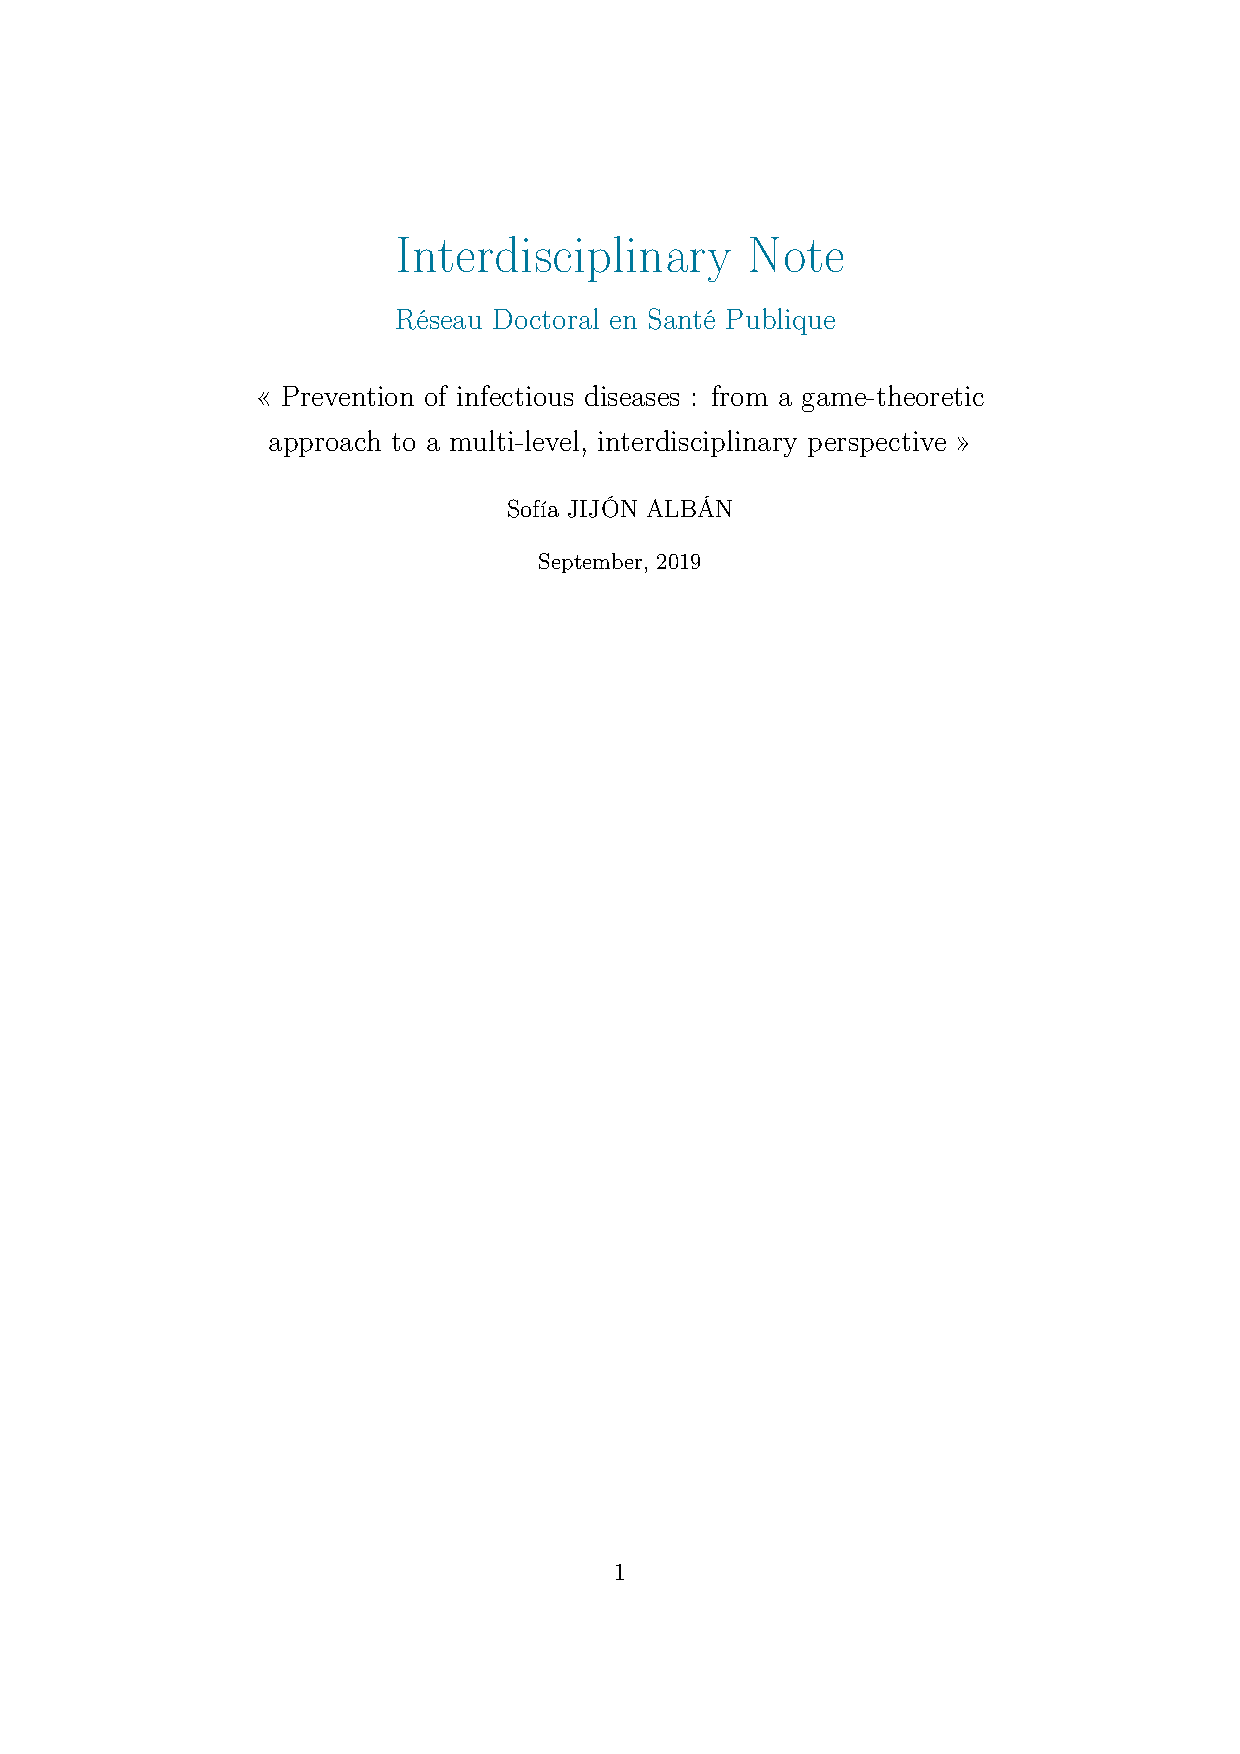
\includepdf[pages = -,
		frame = false,
		link = true,
		linkname = NID,
		openright = false, 
		offset = 0cm -0.5cm,
		pagecommand = { }]
		{Parts/Documents/NID_EHESP_V2/NID_EHESP.pdf}
%		{DRAFT_FigsAndDocs/NID.pdf}
